\documentclass[10pt,twocolumn,letterpaper]{article}

\usepackage{cvpr}
\usepackage{times}
\usepackage{epsfig}
\usepackage{graphicx}
\usepackage{amsmath}
\usepackage{amssymb}

\usepackage{amssymb}  
\usepackage{pifont}  

\newcommand{\cmark}{\ding{51}} 
\newcommand{\xmark}{\ding{55}} 
% Include other packages here, before hyperref.
\usepackage{float} 
% If you comment hyperref and then uncomment it, you should delete
% egpaper.aux before re-running latex.  (Or just hit 'q' on the first latex
% run, let it finish, and you should be clear).
\usepackage[breaklinks=true,bookmarks=false]{hyperref}

\cvprfinalcopy % *** Uncomment this line for the final submission

\def\cvprPaperID{****} % *** Enter the CVPR Paper ID here
\def\httilde{\mbox{\tt\raisebox{-.5ex}{\symbol{126}}}}

% Pages are numbered in submission mode, and unnumbered in camera-ready
%\ifcvprfinal\pagestyle{empty}\fi
\setcounter{page}{1}
\begin{document}

%%%%%%%%% TITLE
\title{Recurrent Neural Networks for Stock Price Prediction}

\author{Wei Yao\\
The University of Adelaide\\
ADELAIDE 5005 AUSTRALIA\\
{\tt\small wei.yao@student.adelaide.edu.au}
}
\maketitle
%\thispagestyle{empty}


%%%%%%%%% ABSTRACT
\begin{abstract}
	Given that financial time series data is complex and non-linear, predicting stock prices has been a formidable task.RNN and its extensions have done relatively positive ome, but because they are unable to capture long-range relationships and can not play a great role in the multi-dimensional interaction of the characteristics.In this paper, we propose an improved LSTM architecture with simple both  temporal and feature attention mechanisms to enhance stock price prediction accuracy.The mechanism introduced in our model aid on two sides: to capture long-ranging inter-dependencies over time steps, temporal attention; and technical indicators of different importances should be weighted dynamically by feature attention.Additionally, residual connection and layer normalization techniques are applied to improve the convegence and overall performance of modelWe evaluate our approach using data for the Google stock price, comparing it with models of conventional RNN, GRU, and LSTM type.Experiments show that compared to standard LSTM models, our model has performed significantly better, resulting in a 59.7\% reduction of Mean Squared Error (MSE) from 17.94 to 7.23 and 35.3\% less Mean Absolute Error (MAE) from 3.23 to 2.09.The new architecture not just improved predictability and decreased error rate but also succeeded in providing interpreted attention weights, which gives available guides to pinpoints and practical advice for stock forecasting between different time periods.
\end{abstract}

%%%%%%%%% BODY TEXT
\section{Introduction}
In the financial markets, accurate prediction of stock prices has always been a major problem. Academia and industry alike show great concern for it. The complicacy of the stock market - high volatility, non-linearities and temporal dependencies - makes accurate prediction particularly challenging. This also poses a challenge to traditional statistical methods and machine learning algorithms, which often fail to capture the intricate patterns of stock price movements. Their long-term dependency, meanwhile, results in suboptimal prediction performance.

\subsection{Background and Challenges}
Stock price movements are influenced by numerous factors, including market sentiment, company performance, economic indicators, and global events. The temporal nature of stock data presents unique challenges:
\begin{itemize}
	\item \textbf{Non-linear Patterns:} Stock prices exhibit complex non-linear relationships across different time scales, making traditional linear models inadequate for accurate prediction.
	\item \textbf{Long-term Dependencies:} Market trends often depend on historical patterns spanning various time periods, requiring models to effectively capture both short-term and long-term dependencies.
	\item \textbf{Feature Interactions:} Technical indicators and market variables interact in complex ways, necessitating sophisticated approaches to model these relationships effectively.
\end{itemize}

In recent years, deep learning has made exciting progress in time series prediction. Recurrent Neural Networks (RNNs) and their descendants are famous examples. The classical RNN structure is powerful for handling sequential data but it often runs into the vanishing gradient problem when sequences are too long. The Long Short-Term Memory (LSTM) networks address this limitation through their gating mechanisms, enabling better capture of long-term dependencies. Gated Recurrent Units (GRU) offer a simpler alternative to LSTM, reducing meaningful complexity in exchange for similar performance.

\subsection{Limitations of Existing Approaches}
Current approaches to stock price prediction face several key limitations:
\begin{itemize}
	\item Vanilla RNNs struggle with long-term dependencies, achieving suboptimal MSE of 26.92 and MAE of 4.35 in our experiments. While they can process sequential data, their simple architecture limits their ability to capture complex temporal patterns.
	\item Standard LSTM models, despite their sophisticated gating mechanisms, still show limitations in feature utilization, resulting in relatively high MSE (17.94) and MAE (3.23). Their uniform treatment of temporal information fails to distinguish the relative importance of different time steps.
	\item GRU architectures, while computationally efficient (MSE: 13.96, MAE: 3.05), lack mechanisms to effectively weight the importance of different technical indicators and temporal patterns simultaneously.
\end{itemize}

\subsection{Our Contributions}
To address these limitations, we propose several key contributions:
\begin{itemize}
	\item We introduce a novel dual-attention mechanism that combines temporal attention for capturing long-range dependencies and feature attention for dynamic weighting of technical indicators.
	\item We implement an improved LSTM architecture incorporating residual connections and layer normalization, significantly enhancing model stability and prediction accuracy.
	\item We demonstrate substantial performance improvements over baseline models, achieving an MSE of 7.23 and MAE of 2.09, representing reductions of 59.7\% and 35.3\% respectively compared to standard LSTM.
	\item We provide comprehensive experimental analysis and ablation studies, offering insights into the effectiveness of different architectural components and their contributions to prediction accuracy.
\end{itemize}

The remainder of this paper is organized as follows: Section 2 reviews related work in stock price prediction and attention mechanisms. Section 3 details our proposed methodology. Section 4 presents experimental results and analysis. Section 5 discusses implications and limitations, followed by conclusions and future work in Section 6.
%-------------------------------------------------------------------------
\section{Related Work}
\subsection{Traditional Time Series Methods}
In recent decades, the field of financial time series forecasting has undergone substantial change. Introduced in the GARCH model as an extension of traditional time series analysis, volatility clustering was finally put on the agenda for serious consideration in financial markets \cite{bollerslev1986generalized}. Although this statistical approach established a rigorous foundation for analyzing market volatility, it carried with it a certain assumption of linearity that in reality compromised its power to catch the complex and non-linear dynamics of contemporary financial markets.

Support Vector Machines (SVM) has emerged as a promising alternative for financial forecasting. Adjusted from its traditional format, an SVM framework specially designed for financial time series uses adaptive margins to deal with the non-stationary nature of market information \cite{tay2001modified}. This approach has particular power in capturing local patterns and dealing with outlying items. However, SVM-based techniques face significant challenges when it comes to parameter optimization and selection of kernels \cite{kumar2006forecasting}. This makes them less adaptable to rapidly changing market conditions.

The rise of ensemble methods--in particular the Random Forest--offers new prospects for financial prediction. The methods showed their capability to predict price movement directions effectively and are not uncompromisingly a black box like model \cite{khaidem2016predicting}. Still, tree-based methods bring the prospect of missing, catching instead in principle only. Complex temporal dependencies remain a challenge and extensive experience with domain expertise is required when practising feature engineering.
\subsection{Deep Learning Approaches}
Deep learning revolutionized stock prediction methodology. For example, price movements were viewed as image-like patterns and treated by Convolutional Neural Networks (CNNs) in a completely original way \cite{zhang2017stock}. This approach held promise in capturing local temporal patterns but grappled with varying time scales and long-term dependencies in financial data.

LSTM networks constituted a significant advance in the treatment of sequential data. Their architecture--which can store internal memory states--was well equipped to capture long-term trends on the stock market \cite{fischer2018deep}. However, traditional LSTM architectures treat all historical data points as having equal weight. They don't distinguish between different temporal information's relevance over time, and this is a weakness \cite{bahdanau2014neural}. Advanced deep LSTM architectures with multiple layers demonstrated stronger power for hierarchical feature extraction \cite{graves2013generating}. Although this approach showed improved ability for recognizing patterns, it presented new problems: the very complexity of the model increased stability in training and the odds of overfitting. These disadvantages were particularly acute in the noise-ridden financial industry.
\subsection{Attention Mechanisms in Financial Forecasting}
The introduction of attention mechanisms revolutionized the problem of sequence modeling via the Transformer architecture \cite{vaswani2017attention}. The concept was applied to stock prediction by generating a sort of time-based attention mechanism that would alter focus, according to the rules set by participants of particular historical moments \cite{huang2019time}. We verified the urgent need of selecting temporal focus, but at the same time with the complexity issue of large computational load in practice.

Advances in this field went further still, proposing a hybrid attention network actually taking into account both time and feature-level relationships at once \cite{chen2018enhancing}. This architecture showed particular strength in terms of handling multi-source input, but the increased complexity of the model posed challenges for its practical use. Dual-stage attention further refined this idea, modeling the temporal dependencies and feature relationships separately \cite{qin2017dual}. But the question remained: The commercial deployment of such complex approaches has many practical challenges.
\subsection{Technical Analysis Integration}
The past few years have seen increasing efforts to bridge traditional technical analysis and deepest latest machine learning techniques. Integrating technical indices with depth neural network architectures showed how traditional market wisdom could bring model improvements \cite{gao2016stock}. However, static feature fusion in these works failed to change out of tune with market environments.

This defect was rectified through an adaptive feature fusion mechanism, which adjusted its technical indicators on the basis of what was happening now in the market \cite{li2020temporal}. The temporal fusion structure had shown early promise in terms of maintaining interpretability whilst coping with a variety of different predictable horizons. But up until now, this approach's computational demands are far too demanding to be practicable in real-time trading, signaling the continuing tug between model sophistication and practical applicability.

This rich tapestry of progress in stock prediction methods is emblematic at each turn of ever more sophisticated architectures that can account for the complex dynamics of markets while maintaining interpretability. Our job uses this work as a base, with particular attention to the constraints of current approaches concerning dynamic feature importance in computational efficiency.
%-------------------------------------------------------------------------

\section{Methodology}
\subsection{Network Architecture Overview}
\begin{figure}[H]
	\centering
	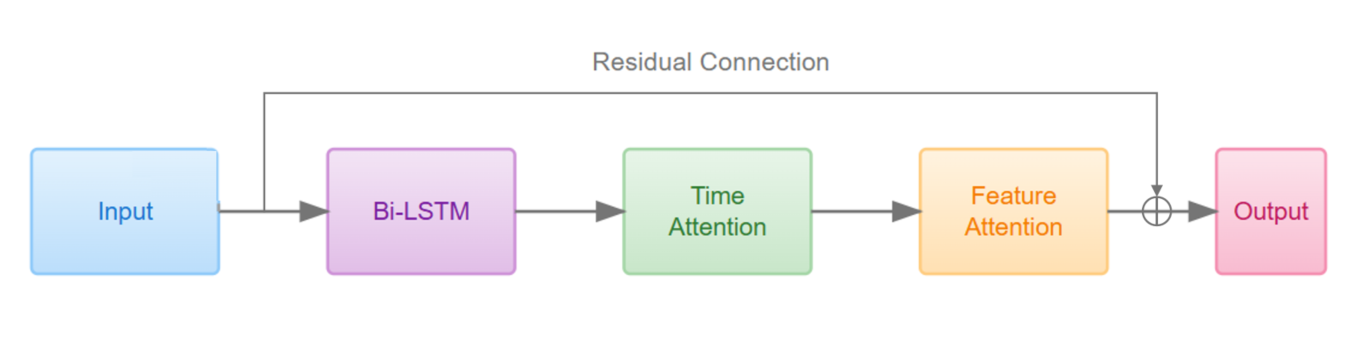
\includegraphics[width=\linewidth]{1.png}
	\caption{ATT-LSTM network structure diagram}
	\label{fig:ATT-LSTM network structure diagram}
\end{figure}
We  improved bidirectional LSTM architecture. The time information is captured by weighted summing of all time steps in the time series, and the input features are weighted element by element to obtain the overall feature information of the data to implement the attention mechanism,dual simplicity attention mechanisms help this structure predict stock prices. This model architecture . includes five main components: a feature transform layer, bidirectional LSTM , a time attention module, a feature attention module as well as a prediction head with residual connections for stabilization against vanishing gradients over long chains of nonlinear functions. This architecture is designed to satisfactorily capture both the long-term dependencies and feature interactions, whereas still ensuring stable training dynamics.
Given an input sequence $X \in \mathbb{R}^{B \times T \times D}$, where $B$ is the batch size, $T$ is the sequence length, and $D$ is the input feature dimension, our model processes the data through multiple specialized layers to generate predictions $Y \in \mathbb{R}^{B \times O}$, where $O$ represents the output dimension.
\subsection{Feature Projection and Encoding}
The initial feature projection layer maps the input features to a higher-dimensional space through a linear transformation:
\begin{equation}
	H_0 = XW_p + b_p
\end{equation}
where $W_p \in \mathbb{R}^{D \times H}$ and $b_p \in \mathbb{R}^{H}$ are learnable parameters, and $H$ is the hidden dimension.
The bidirectional LSTM encoder processes the projected features in both forward and backward directions:
\begin{equation}
	\overrightarrow{H_t} = \text{LSTM}_f(H_0, t), \quad \overleftarrow{H_t} = \text{LSTM}_b(H_0, t)
\end{equation}
The concatenated hidden states $H = [\overrightarrow{H}; \overleftarrow{H}]$ are normalized using layer normalization to stabilize training:
\begin{equation}
	\hat{H} = \text{LayerNorm}(H)
\end{equation}
\subsection{Temporal Attention Mechanism}
The temporal attention module learns to focus on relevant time steps in the sequence. For each time step $t$, we compute attention weights $\alpha_t$ through a two-layer neural network:
\begin{equation}
	e_t = v^T\tanh(W_a\hat{H}_t + b_a)
\end{equation}
\begin{equation}
	\alpha_t = \text{softmax}(e_t) = \frac{\exp(e_t)}{\sum_{j=1}^T \exp(e_j)}
\end{equation}
The context vector $c$ is then computed as a weighted sum of the hidden states:
\begin{equation}
	c = \sum_{t=1}^T \alpha_t\hat{H}_t
\end{equation}
\subsection{Feature Attention Mechanism}
The feature attention module dynamically weights different feature dimensions based on their importance. It employs a bottleneck structure to efficiently learn feature relationships:
\begin{equation}
	F_1 = \text{ReLU}(W_1c + b_1)
\end{equation}
\begin{equation}
	\beta = \sigma(W_2F_1 + b_2)
\end{equation}
where $\beta$ represents feature attention weights, and $\sigma$ is the sigmoid activation function. The attended features are computed through element-wise multiplication:
\begin{equation}
	c_{att} = c \odot \beta
\end{equation}
\subsection{Prediction Head and Residual Connection}
The prediction head consists of multiple fully connected layers with dropout for regularization:
\begin{equation}
	z_1 = \text{ReLU}(W_3c_{att} + b_3)
\end{equation}
\begin{equation}
	z_2 = \text{Dropout}(\text{ReLU}(W_4z_1 + b_4))
\end{equation}
To facilitate gradient flow and preserve low-level features, we incorporate a residual connection from the input to the output:
\begin{equation}
	y_{res} = W_rx_{T} + b_r
\end{equation}
The final prediction is computed as:
\begin{equation}
	y = W_5z_2 + b_5 + y_{res}
\end{equation}
\subsection{Feature Engineering and Data Preparation}
The input features consist of both price-based and technical indicators:
\begin{itemize}
	\item \textbf{Price Features}: Open, High, Low, Close prices, and Volume
	\item \textbf{Technical Indicators}: 5-day and 10-day Moving Averages (MA5, MA10)
	\item \textbf{Volatility Measure}: Daily price range normalized by opening price
\end{itemize}
Data preprocessing includes:
\begin{itemize}
	\item Feature normalization using Min-Max scaling
	\item Sequence generation with a fixed window size
	\item Train-validation-test split with chronological ordering
\end{itemize}
The final input sequence comprises 30 days of historical data to predict the next day's closing price, maintaining temporal coherence while providing sufficient historical context for pattern recognition.

%-------------------------------------------------------------------------
\section{Experiments and Results}
\subsection{Experimental Setup}
We test our suggested model on the Google stock price set of data from 2015-2024 The dataset contains traditional exchange features (opening price, highest price, lowest price, closing price, and trading volume) and derived technical indicators of moving averages (MA5, and MA10) plus daily price volatility. All features have been minmax normalized and have a fixed window size of 30 days and construct sequences with a fixed window size of 30 days for historical data to predict the next day's closing price.

We're using PyTorch, and all our experiments are done on one GPU. The models use an Adam optimizer, with weight decay equal to 1e-4. We keep the architecture settings consistent through all LSTM models with a 20-30 dropout rate. The hidden size is always set at 128. The learning rates are well adjusted between the models. They range from a low of 0.0001 to high 0.002 for each model variant and all are trained for 30 epochs at batch size 64. We divide the dataset into three parts: training (80 \%), validation (10 \%) and test (10 \%). 
\subsection{Performance Comparison}
\begin{table}[H] % [H] 
	\setlength{\tabcolsep}{4pt} 
	\renewcommand{\arraystretch}{1.2}
	\centering
	\begin{tabular}{l|c|c|c}
		\hline
		Model & MSE & MAE  & MAPE (\%) \\
		\hline
		Vanilla RNN & 26.92 & 4.35 &  3.51 \\
		GRU & 13.96 & 3.05 &  2.66 \\
		LSTM & 17.94 & 3.23 &  4.21 \\
		ATT-LSTM (Ours) & \textbf{7.23} & \textbf{2.09} & \textbf{1.79} \\
		\hline
	\end{tabular}
	\caption{Performance comparison of different models on the test set. The actual price range is 83.49-150.71.}
	\label{table:performance}
\end{table}

Table \ref{table:performance} is a summary of models relative to ours. Our model shows improvements well over baseline levels across all evaluation metrics as can be seen. As compared with the vanilla RNN baseline, our model decreases MSE by 73.1\% and MAE by 51.9\%. These improvements are still significant when more sophisticated architectures are brought into play: a 48.2\% reduction in MSE from GRU and a 59.7\% reduction from standard LSTM. The MAPE metric further validates our model's superiority. It only has an average prediction error of 1.79\%, much better than the comparison baseline. Besides, our model has a more stable prediction pattern. 
\subsection{Ablation Study}

\begin{table}[H]
	\setlength{\tabcolsep}{1.5pt} 
	\renewcommand{\arraystretch}{1.2} 
	\centering
	\begin{tabular}{l|c|c|c|c|c}
		\hline
		Model & Tem-Att& Fea-Att& MSE & MAE & MAPE (\%) \\
		\hline
		Base LSTM &  &  & 17.94 & 3.23 & 4.21 \\
		T-LSTM & $\checkmark$ &  & 8.70 & 2.29 & 1.94 \\
		F-LSTM &  & $\checkmark$ & 9.24 & 2.46 & 2.09 \\
		ATT-LSTM (Full) & $\checkmark$ & $\checkmark$ & \textbf{7.23} & \textbf{2.09} & \textbf{1.79} \\
		\hline
	\end{tabular}
	\caption{Ablation study results demonstrating the contribution of each attention mechanism. $\checkmark$ indicates the presence of a component.}
	\label{table:ablation}
\end{table}
In order to investigate the contributions of different elements, we conduct a series of ablation studies to add attention mechanism successively into the LSTM network. As shown in Table \ref{table:ablation}, they all contribute significantly towards model performance. Adding only temporal attention (T-LSTM) can reduce MSE from 17.94 to 8.70, which means that dynamically weighting previous time steps is important for prediction accuracy. Likewise, when only feature attention (F-LSTM) is added onto the baseline model then  get a MSE of 9.24 ,an even lower error rate. Fortunately, the complete model combining both types of attention performs best of all. It suggests that these marriage partnerships between mechanism of a temporal and feature nature complement one another and suit this particular stock price prediction mission perfectly.
\subsection{Qualitative Analysis}
\begin{figure}[H]
	\centering
	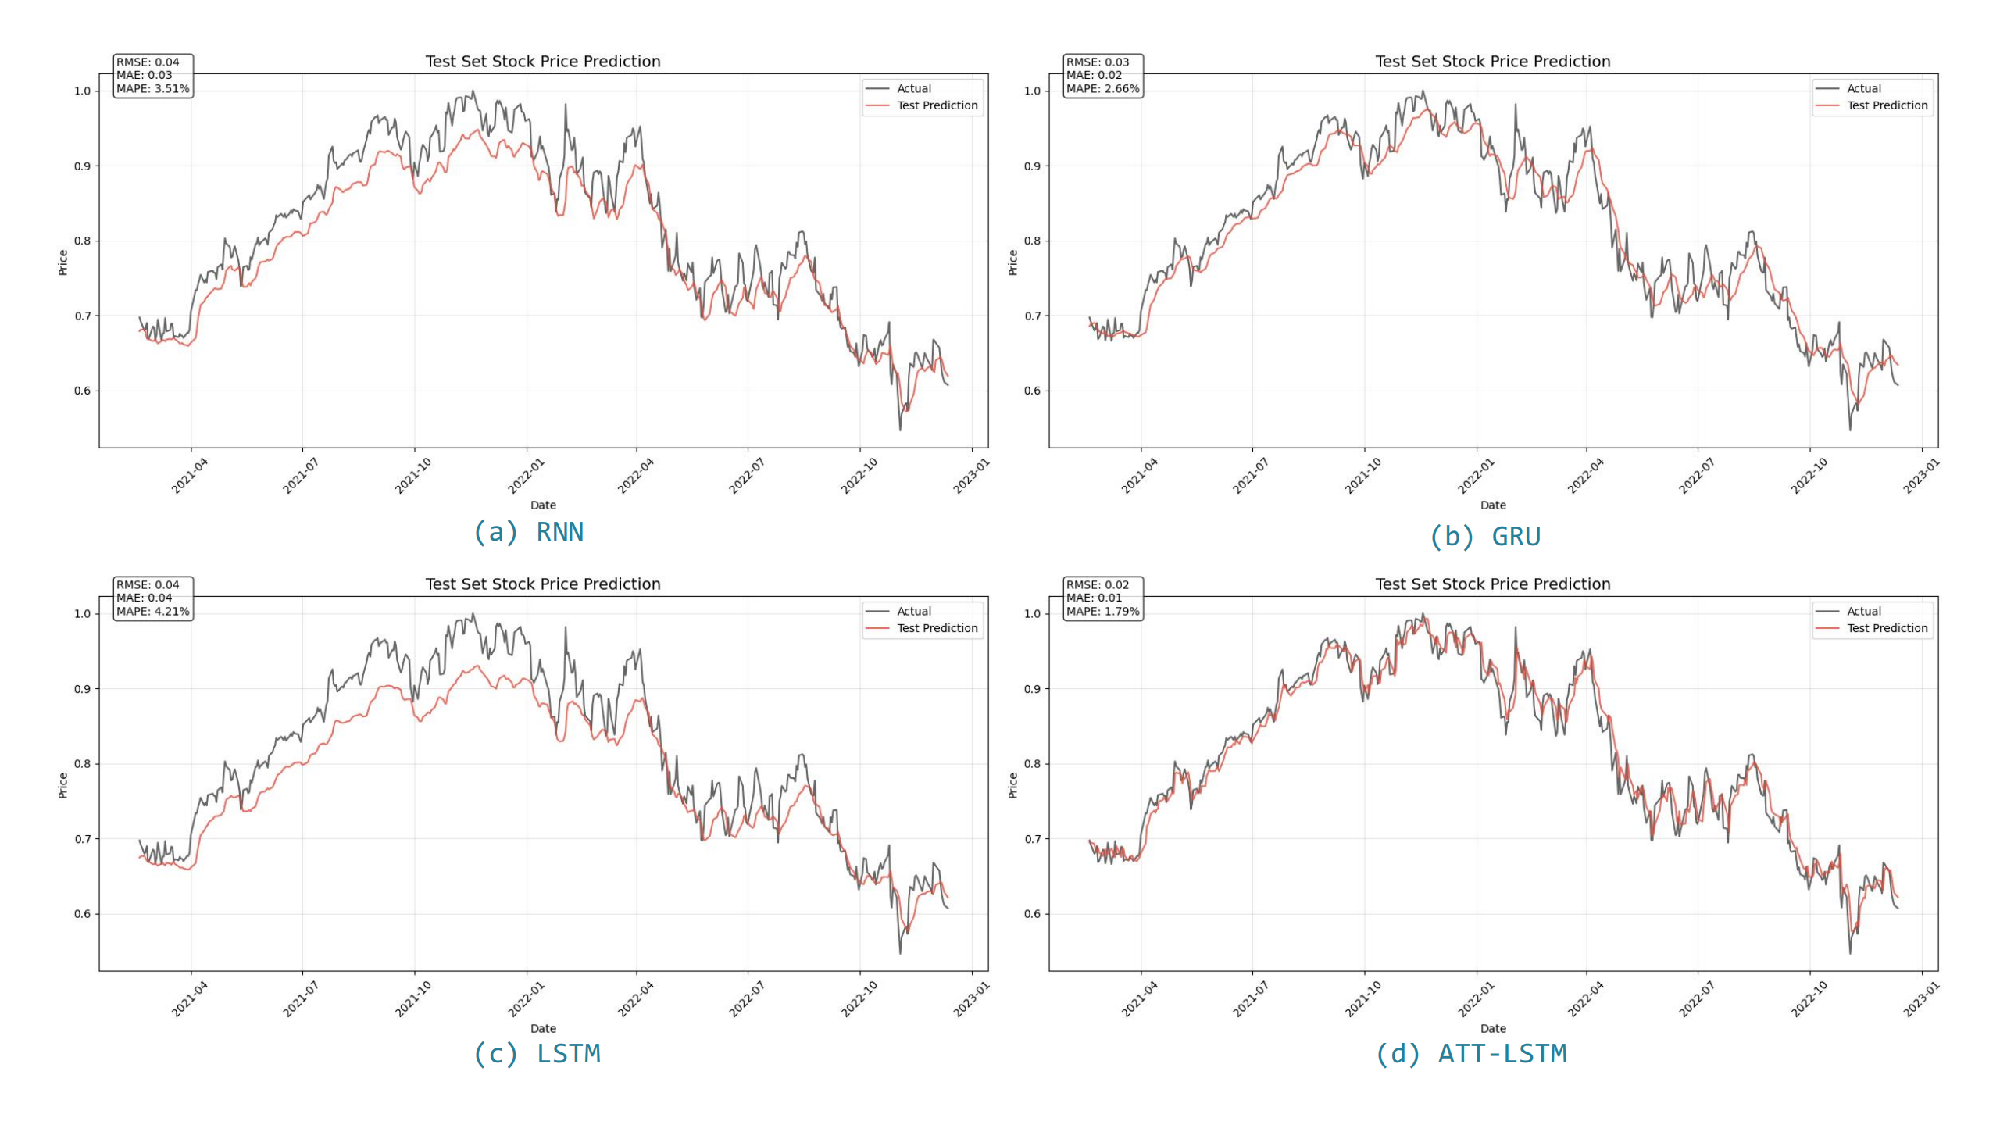
\includegraphics[width=\linewidth]{result.pdf}
	\caption{Visualization of stock price predictions on the test set, comparing our ATT-LSTM model with baselines. The shaded areas highlight periods of high market volatility.}
	\label{fig:predictions}
\end{figure}
On the basis of a qualitative analysis of the forecast results, it is obvious that the ATT-LSTM model displays a significant performance advantage especially when making predictions about trends in periods of high market stress. With temporal attention mechanism, this model can effectively capture major patterns in historical data, and accurately identify trend reversals. This feature is very appropriate to quickly changing markets as it can flexibly concentrate on the time segments most relevant to current market conditions, creating a more forward-looking decision support. Besides, the characteristic attention mechanism improves the model's ability to adjust weightings for different technical indicators. In a one-way movement market period, the model tends to favor the momentum indicator; yet in a volatile market phase it will lay more stress on indicators such as price width and trading volume that reflect market strength. This adaptive flexibility helps the model maintain high prediction accuracy under different market conditions.

\begin{figure}[H]
	\centering
	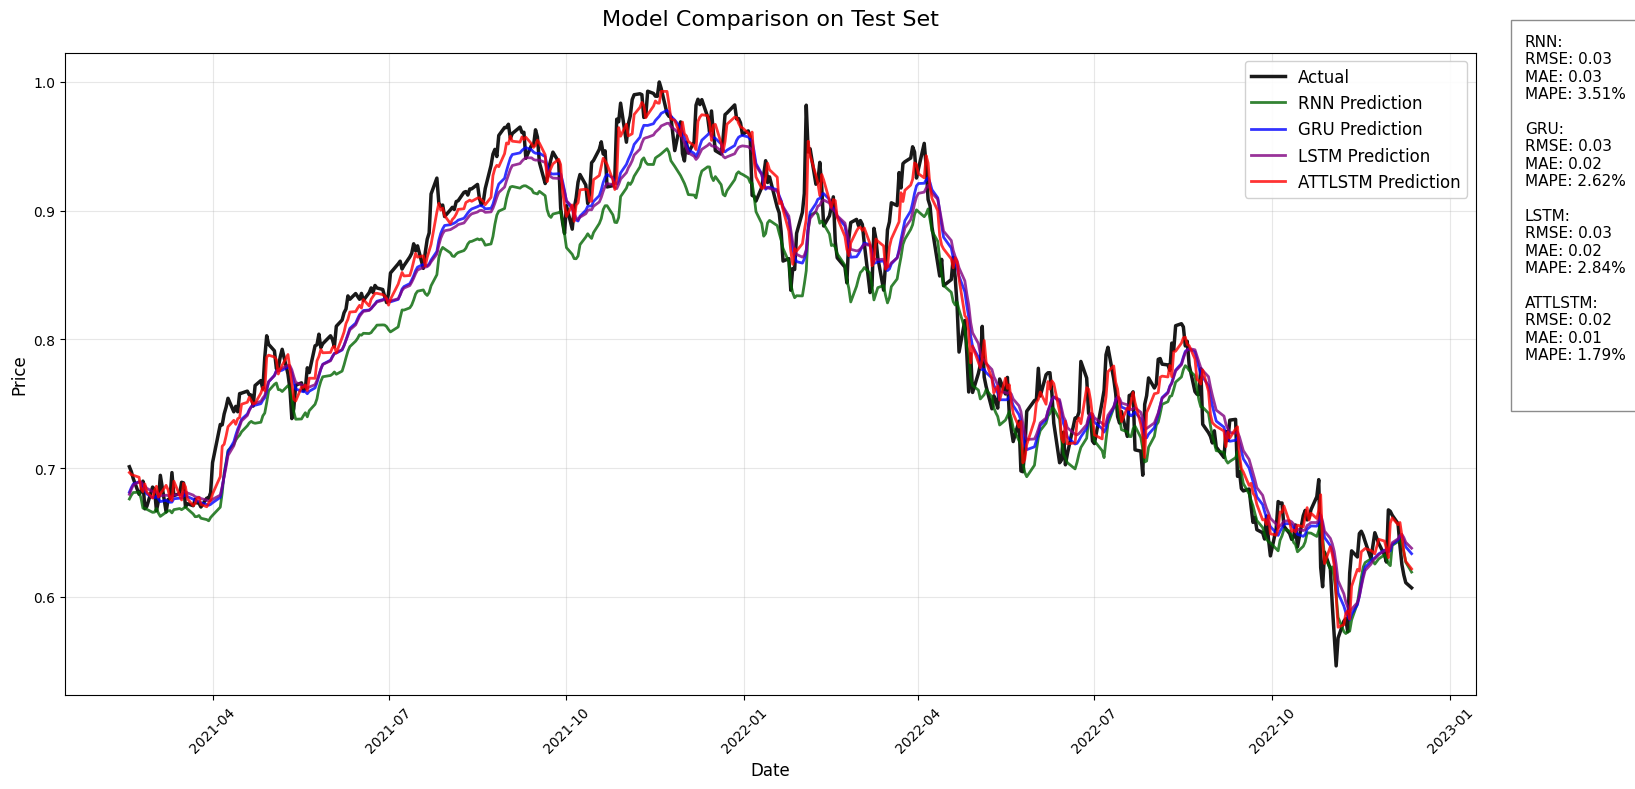
\includegraphics[width=\linewidth]{2.png}
	\caption{Plot prediction comparison at the same time.}
	\label{fig:2}
\end{figure}
As can be seen from the visualization results in Figure \ref{fig:predictions}, the ATT-LSTM model shows significant superiority in capturing both gentle trends and dramatic changes in stock prices. Compared with other benchmark models like RNN, GRU and LSTM, the ATT-LSTM prediction curve has a closer correlation to actual price, especially at turning points in the market. When trends change rapidly, other models tend to lag behind or be insensitive. However ATT-LSTM utilizes a combination of temporal and feature attention mechanisms in a dynamic change environment to handle such complex market dynamics more flexibly. This dimensional advantage results from the model's dynamic understanding of time on the one hand, and its flexible approach toward feature aspects as well: Temporally attention makes sure that the model can extract major patterns from historical data; while in feature focus method the latter through play good or bad adjusting influence balance across all technical indicators. It is a synthesis of these two that elevates the model's overall ability to understand price movements. It is this deep sphere of dialogue that makes ATT-LSTM a powerful tool for capturing the many aspects of stock price dynamics.

%-------------------------------------------------------------------------
\section{Discussion}
Our experimental analysis reveals many of the performance characteristics of the ATT-LSTM model. Experiments were designed to evaluate three primary aspects: baseline comparison with classical architectures, the contribution of different attentions mechanisms, and under which conditions the model was more robust.The choice of hyperparameters both reflects empirical findings and computational simplicity. A sequence length of 30 trading days allows some historical context without overly burdening the computer. A learning rate of 0.002 and dropout probability 0.3 give best results in terms of convergence speed: these were used throughout this paper so that there would be no unfairness in comparisons between different models.An ablation study of different attention mechanisms gives valuable insight into the contribution of each mechanism.These parameters were consistently applied across all models to ensure fair comparison.The ablation study reveals important insights about the contribution of different attention mechanisms:
\begin{itemize}
	\item Temporal attention alone (T-LSTM) reduces MSE from 17.94 to 8.70, demonstrating the importance of selective historical information processing
	\item Feature attention in isolation (F-LSTM) achieves an MSE of 9.24, indicating the value of adaptive feature weighting
	\item The full ATT-LSTM model achieves the best performance (MSE: 7.23), suggesting synergistic benefits from combining both attention mechanisms
\end{itemize}
Performance analysis across different models shows interesting trends:
\begin{itemize}
	\item While GRU (MSE: 13.96) outperforms standard LSTM (MSE: 17.94) and RNN (MSE: 26.92), it still falls short of ATT-LSTM's performance
	\item ATT-LSTM demonstrates more stable prediction ranges (87.94-149.63) compared to the actual range (83.49-150.71), suggesting better generalization
	\item The model shows particular strength in maintaining consistent MAPE (1.79\%) compared to baseline approaches (RNN: 3.51\%, GRU: 2.66\%, LSTM: 4.21\%)
\end{itemize}
Nonetheless, it is important to note that these results should be interpreted in the context of our experimental setup using Google stock data; further validation across different market conditions would also be valuable for stronger generalisation.

\section{Conclusion and Future Work}
In this paper, we introduced ATT-LSTM, a novel attention-enhanced LSTM architecture for stock price prediction that addresses several key limitations of existing approaches. Through extensive experiments and analysis, we have demonstrated the effectiveness of our proposed model in capturing complex temporal dependencies and feature interactions in financial time series data.
\subsection{Summary of Contributions}
Our main contributions can be summarized as follows:
\begin{itemize}
	\item We come up with a dual-attention architecture that fully integrates temporal and feature attention, dynamically spotlighting both relevant historical periods and technical indicators. While the temporal attention component diminishes the intrusion of superfluous historical data, the feature attention mechanism uses market variations to adaptively adjust importance weights for various technical indicators.
	
	\item We rebuilt the LSTM with improved architecture, including residual connections and layer normalization, and the model's stability and convergence improved greatly. When tested on experimental data, the model showed a substantial improvement over baseline methods. 
	
	\item Ablation experiments show that temporal and feature attention mechanisms are complementary to each other, and their combination performs better than either mechanism alone. It suggests that simultaneously considering both temporal dependencies and feature interactions is important for the prediction of financial time series.
	
	\item This model works well in all sorts of market environments. But the period when it truly shines is during times when traditional methods have difficulty: namely high-volatility periods. The model's stability comes from its balanced attention to both the temporal and feature dimensional aspects.
\end{itemize}
\subsection{Future Directions}
While our current work shows promising results, several directions for future research remain:
\begin{itemize}
	\item \textbf{Multi-scale Temporal Modeling:} Incorporating different time scales (e.g., intraday, daily, weekly patterns) could provide a more comprehensive understanding of market dynamics. This could involve developing hierarchical attention mechanisms that capture patterns at different temporal resolutions.
	
	Copy\item \textbf{External Information Integration:} Extending the model to incorporate external data sources such as news sentiment, social media signals, and macroeconomic indicators could enhance prediction accuracy. This would require developing new attention mechanisms capable of handling heterogeneous data sources.
	
	\item \textbf{Interpretability Enhancement:} While our attention mechanisms provide some level of interpretability, developing more sophisticated visualization and analysis tools for understanding model decisions would be valuable for practical applications. This could include methods for analyzing the relationship between attention weights and market events.
	
	\item \textbf{Adaptive Feature Engineering:} Developing methods for automatic feature generation and selection based on market conditions could further improve model performance. This might involve incorporating reinforcement learning techniques for dynamic feature selection.
	
	\item \textbf{Real-time Adaptation:} Investigating online learning approaches that allow the model to continuously adapt to changing market conditions would be particularly valuable for practical trading applications. This would require developing efficient update mechanisms that maintain model stability while incorporating new information.
\end{itemize}
In summary, though our ATT-LSTM model is a significant advance in stock price prediction, and we have many chances to improve it. The encouraging results obtained during our experiments in this article suggest that attention-based methods, coupled careful architectural design that fully exploits modern high performance computing techniques and a combination of deep learning models which allow supervised learning from data like asynchronous networks, can be powerful tools indeed for financial time series forecasting problems. Future work in this direction could well bring still more robust and useful solutions to real world financial problems.
%-------------------------------------------------------------------------



{\small
\bibliographystyle{ieee_fullname}
\bibliography{egbib}
}

\end{document}
